\documentclass[border=3pt]{standalone}
% Preâmbulo compartilhado pelos diagramas TikZ da aula 14 (SLAM com EIF)
\usepackage[T1]{fontenc}
\usepackage[utf8]{inputenc}
\usepackage{lmodern}
\usepackage{amsmath}
\usepackage{xcolor}
\usepackage{tikz}
\usetikzlibrary{arrows.meta,angles,quotes,decorations.pathmorphing,decorations.pathreplacing,calc,
                positioning,shapes.geometric,shapes.misc,backgrounds,fit,
                math}

% Paleta (mesma dos SVGs originais)
\definecolor{dblue}{HTML}{2A5B8C}
\definecolor{dorange}{HTML}{B3541E}
\definecolor{dgreen}{HTML}{4A7C59}
\definecolor{dred}{HTML}{9C4B4B}
\definecolor{dcream}{HTML}{F4F1EA}
\definecolor{dshade}{HTML}{DDD7C9}

% Função gaussiana (não normalizada por padrão de escala visual)
\pgfmathdeclarefunction{gauss}{3}{%
  \pgfmathparse{1/(#3*sqrt(2*pi))*exp(-((#1-#2)^2)/(2*#3^2))}%
}

% Estilos comuns (prefixo d... para não colidir com chaves internas do pgf)
\tikzset{
  >={Stealth[length=2mm]},
  dguide/.style={gray!55, dashed, line width=0.4pt},
  daxis/.style={gray!60, line width=0.7pt, ->},
  dbody/.style={fill=black!3, draw=black!80, line width=1pt},
  dacc/.style={draw=dblue, line width=1pt},
  dlbl/.style={black!55, font=\small},
  dsub/.style={black!45, font=\footnotesize},
  dstate/.style={circle, draw=black!80, fill=dcream, line width=1pt,
                 minimum size=17mm, font=\large, inner sep=1pt},
  dobs/.style={circle, draw=black!80, fill=dshade, line width=1pt,
               minimum size=14mm, font=\large, inner sep=1pt},
  dbox/.style={rounded corners=2pt, draw=black!80, fill=dcream, line width=1pt,
               align=center, inner sep=6pt},
  dop/.style={circle, draw=black!80, fill=white, line width=1pt,
              minimum size=6mm, inner sep=0pt, font=\small},
  dtrans/.style={->, dblue, line width=1pt},
  dmeas/.style={->, dorange, line width=1pt},
  dcurve/.style={line width=1pt, dblue},
  dcurveb/.style={line width=1.4pt, dorange},
}

\begin{document}
\hyphenpenalty=10000 \exhyphenpenalty=10000 \tolerance=9999 \emergencystretch=3em
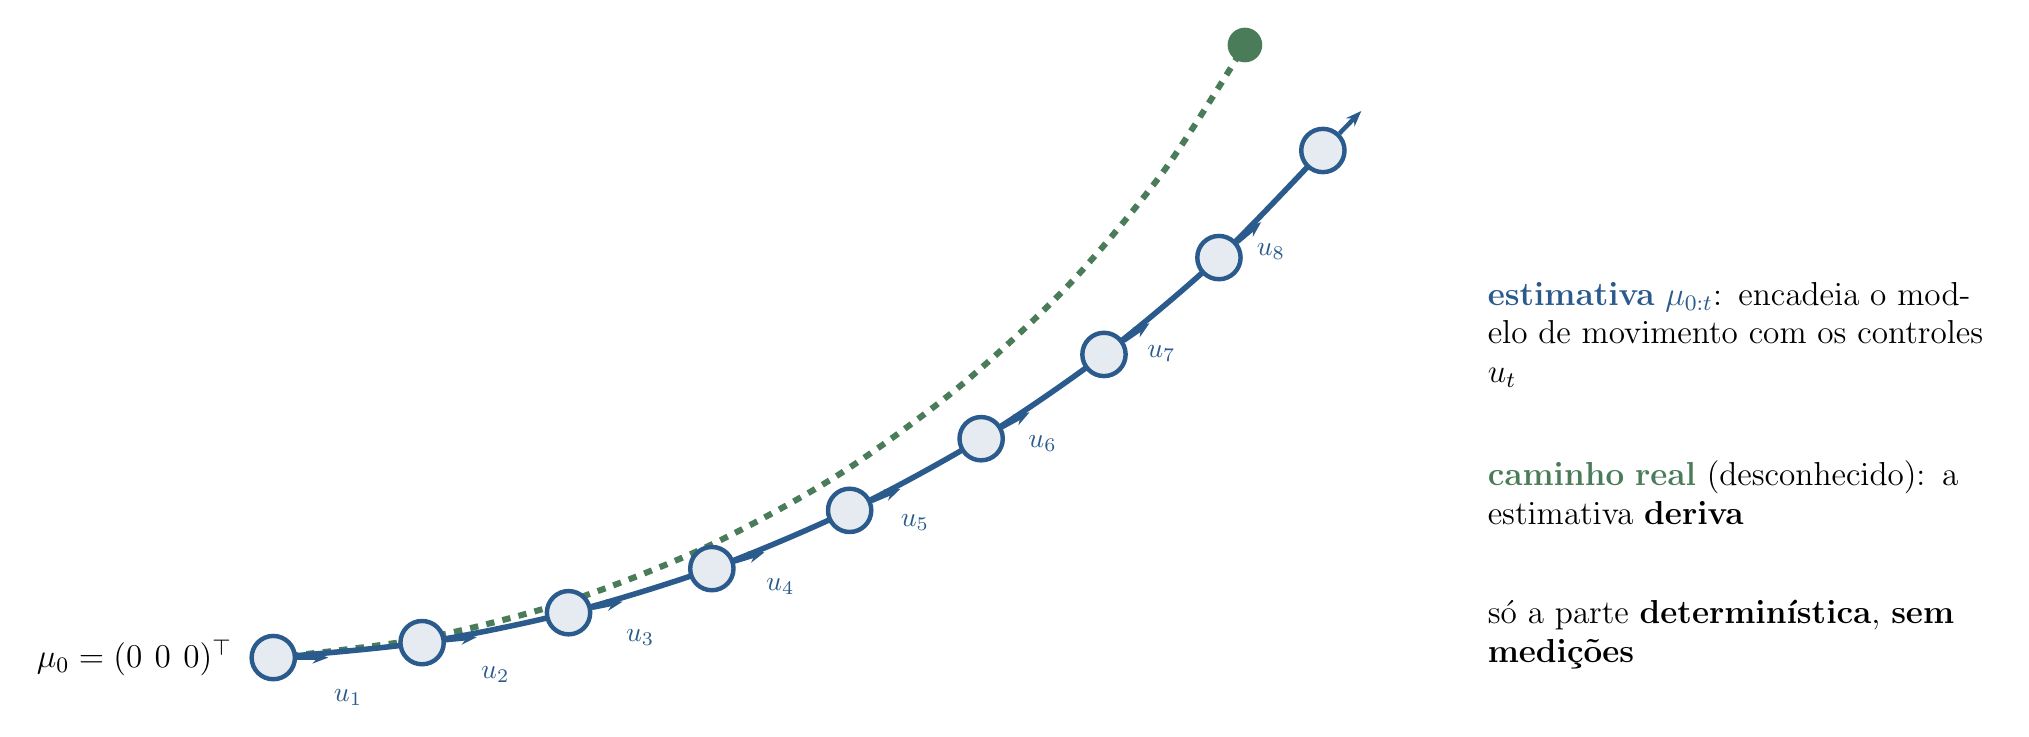
\begin{tikzpicture}[x=1cm,y=1cm]
\tikzset{p/.style={circle, draw=dblue, fill=dblue!12, line width=1.6pt, minimum size=0.55cm}}
\draw[dgreen, dashed, line width=2.2pt, smooth] plot coordinates {(0.90,1.50) (2.79,1.74) (4.63,2.21) (6.39,2.90) (8.06,3.81) (9.60,4.93) (10.99,6.22) (12.21,7.68) (13.24,9.28)}; \fill[dgreen] (13.24,9.28) circle (0.22);
\draw[dblue, line width=2.0pt, smooth] plot coordinates {(0.90,1.50) (2.79,1.69) (4.65,2.07) (6.47,2.63) (8.22,3.37) (9.89,4.28) (11.45,5.35) (12.91,6.58) (14.23,7.94)};
\node[p] (e0) at (0.90,1.50) {}; \draw[->, line width=1.6pt, draw=dblue] (e0) -- ++(0.0:0.7);
\node[p] (e1) at (2.79,1.69) {}; \draw[->, line width=1.6pt, draw=dblue] (e1) -- ++(5.7:0.7);
\node[p] (e2) at (4.65,2.07) {}; \draw[->, line width=1.6pt, draw=dblue] (e2) -- ++(11.5:0.7);
\node[p] (e3) at (6.47,2.63) {}; \draw[->, line width=1.6pt, draw=dblue] (e3) -- ++(17.2:0.7);
\node[p] (e4) at (8.22,3.37) {}; \draw[->, line width=1.6pt, draw=dblue] (e4) -- ++(22.9:0.7);
\node[p] (e5) at (9.89,4.28) {}; \draw[->, line width=1.6pt, draw=dblue] (e5) -- ++(28.6:0.7);
\node[p] (e6) at (11.45,5.35) {}; \draw[->, line width=1.6pt, draw=dblue] (e6) -- ++(34.4:0.7);
\node[p] (e7) at (12.91,6.58) {}; \draw[->, line width=1.6pt, draw=dblue] (e7) -- ++(40.1:0.7);
\node[p] (e8) at (14.23,7.94) {}; \draw[->, line width=1.6pt, draw=dblue] (e8) -- ++(45.8:0.7);

\node[font=\normalsize, text=dblue, fill=white, inner sep=1pt] at (1.85,0.99) {$u_{1}$};
\node[font=\normalsize, text=dblue, fill=white, inner sep=1pt] at (3.72,1.28) {$u_{2}$};
\node[font=\normalsize, text=dblue, fill=white, inner sep=1pt] at (5.56,1.75) {$u_{3}$};
\node[font=\normalsize, text=dblue, fill=white, inner sep=1pt] at (7.34,2.40) {$u_{4}$};
\node[font=\normalsize, text=dblue, fill=white, inner sep=1pt] at (9.05,3.22) {$u_{5}$};
\node[font=\normalsize, text=dblue, fill=white, inner sep=1pt] at (10.67,4.22) {$u_{6}$};
\node[font=\normalsize, text=dblue, fill=white, inner sep=1pt] at (12.18,5.36) {$u_{7}$};
\node[font=\normalsize, text=dblue, fill=white, inner sep=1pt] at (13.57,6.66) {$u_{8}$};

\node[font=\large\bfseries, anchor=east] at (0.5,1.5) {$\mu_0=(0\ 0\ 0)^{\top}$};
\node[font=\large, anchor=west, text width=6.4cm] at (16.2,5.6) {\textcolor{dblue}{\textbf{estimativa} $\mu_{0:t}$}: encadeia o modelo de movimento com os controles $u_t$};
\node[font=\large, anchor=west, text width=6.4cm] at (16.2,3.6) {\textcolor{dgreen}{\textbf{caminho real}} (desconhecido): a estimativa \textbf{deriva}};
\node[font=\large, anchor=west, text width=6.4cm] at (16.2,1.8) {só a parte \textbf{determinística}, \textbf{sem medições}};
\end{tikzpicture}
\end{document}
